\subsection{Torque Measurement Apparatus (In Progress)}

A torque measurement system based on ASTM F2213 is under development. While a prototype was fabricated under the supervision of Dr. Nichols and prior students, detailed calibration, operational workflow, and data acquisition methods are still being finalized. The system is expected to allow both qualitative torque threshold assessments and quantitative torque calculation by assessing rotational displacement under a known static field. This device is shown in figure \ref{fig:torqueDevice}.


\begin{figure}[H]
	\centering
	\begin{minipage}[b]{0.48\textwidth}
		\centering
		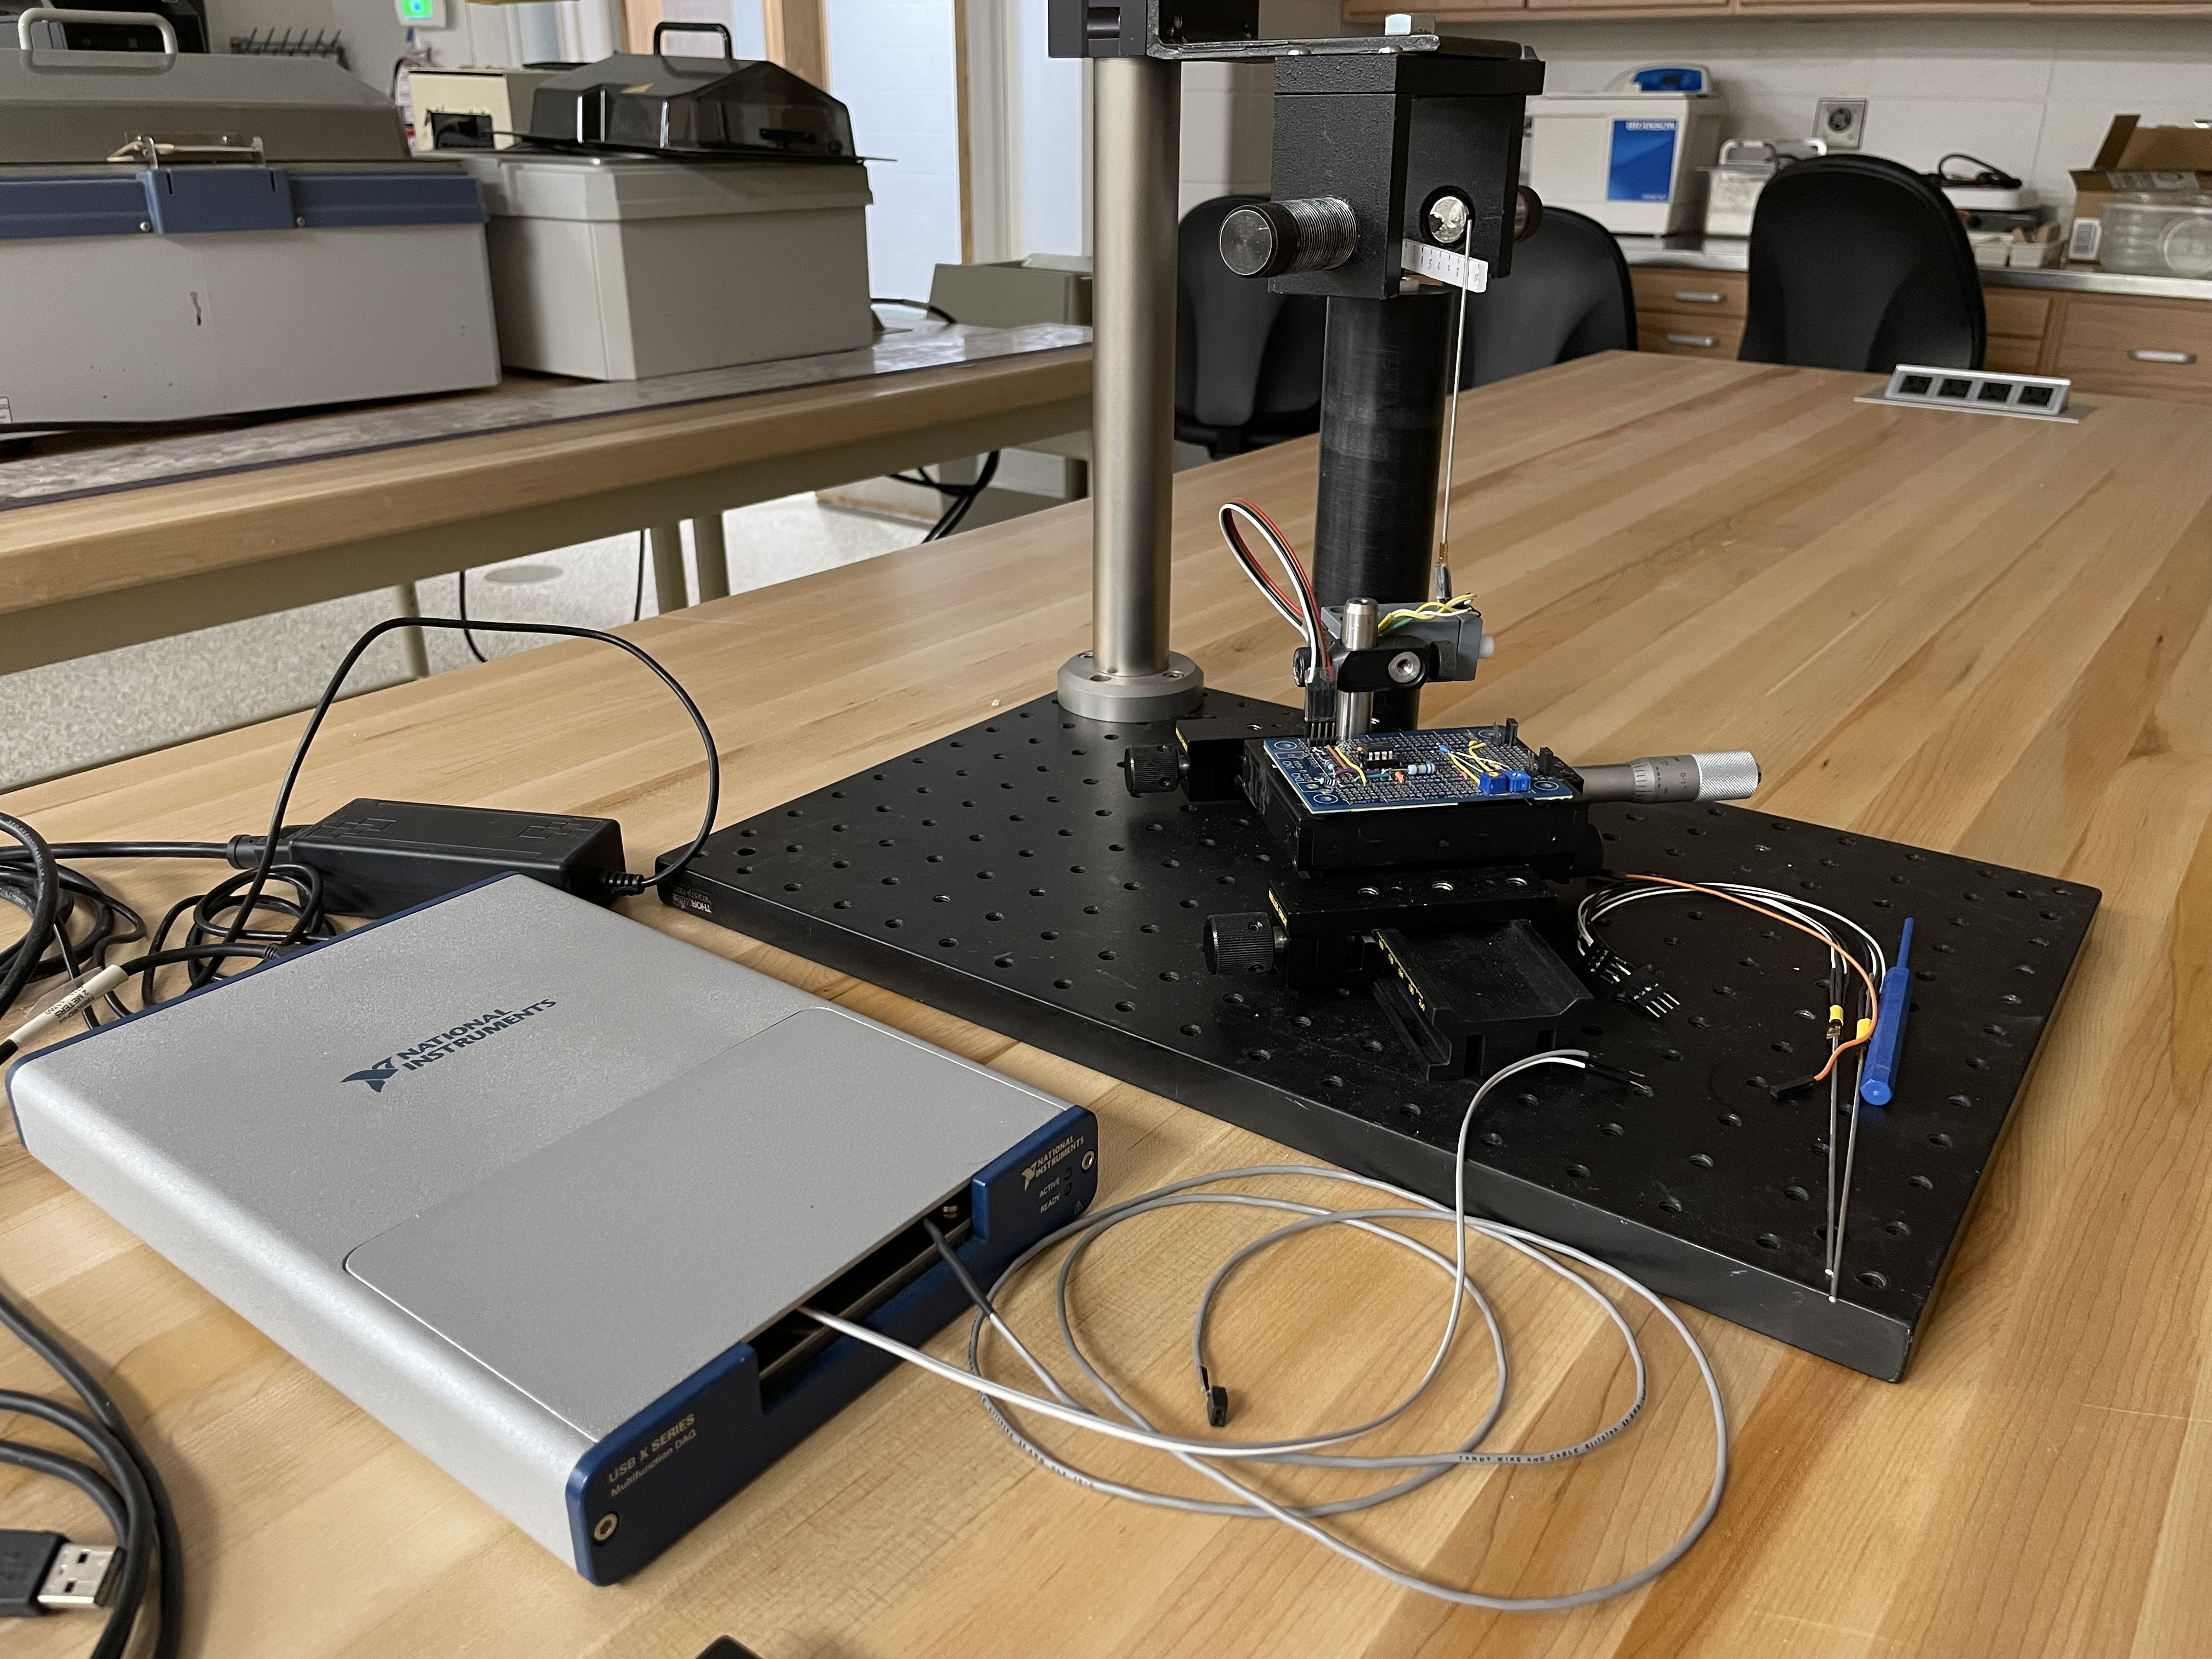
\includegraphics[width=\textwidth]{Assests/torquesDev.jpg}
		\subcaption{Current torque measurement device}
		\vspace{0.95cm}
	\end{minipage}
	\hfill
	\begin{minipage}[b]{0.48\textwidth}
		\centering
		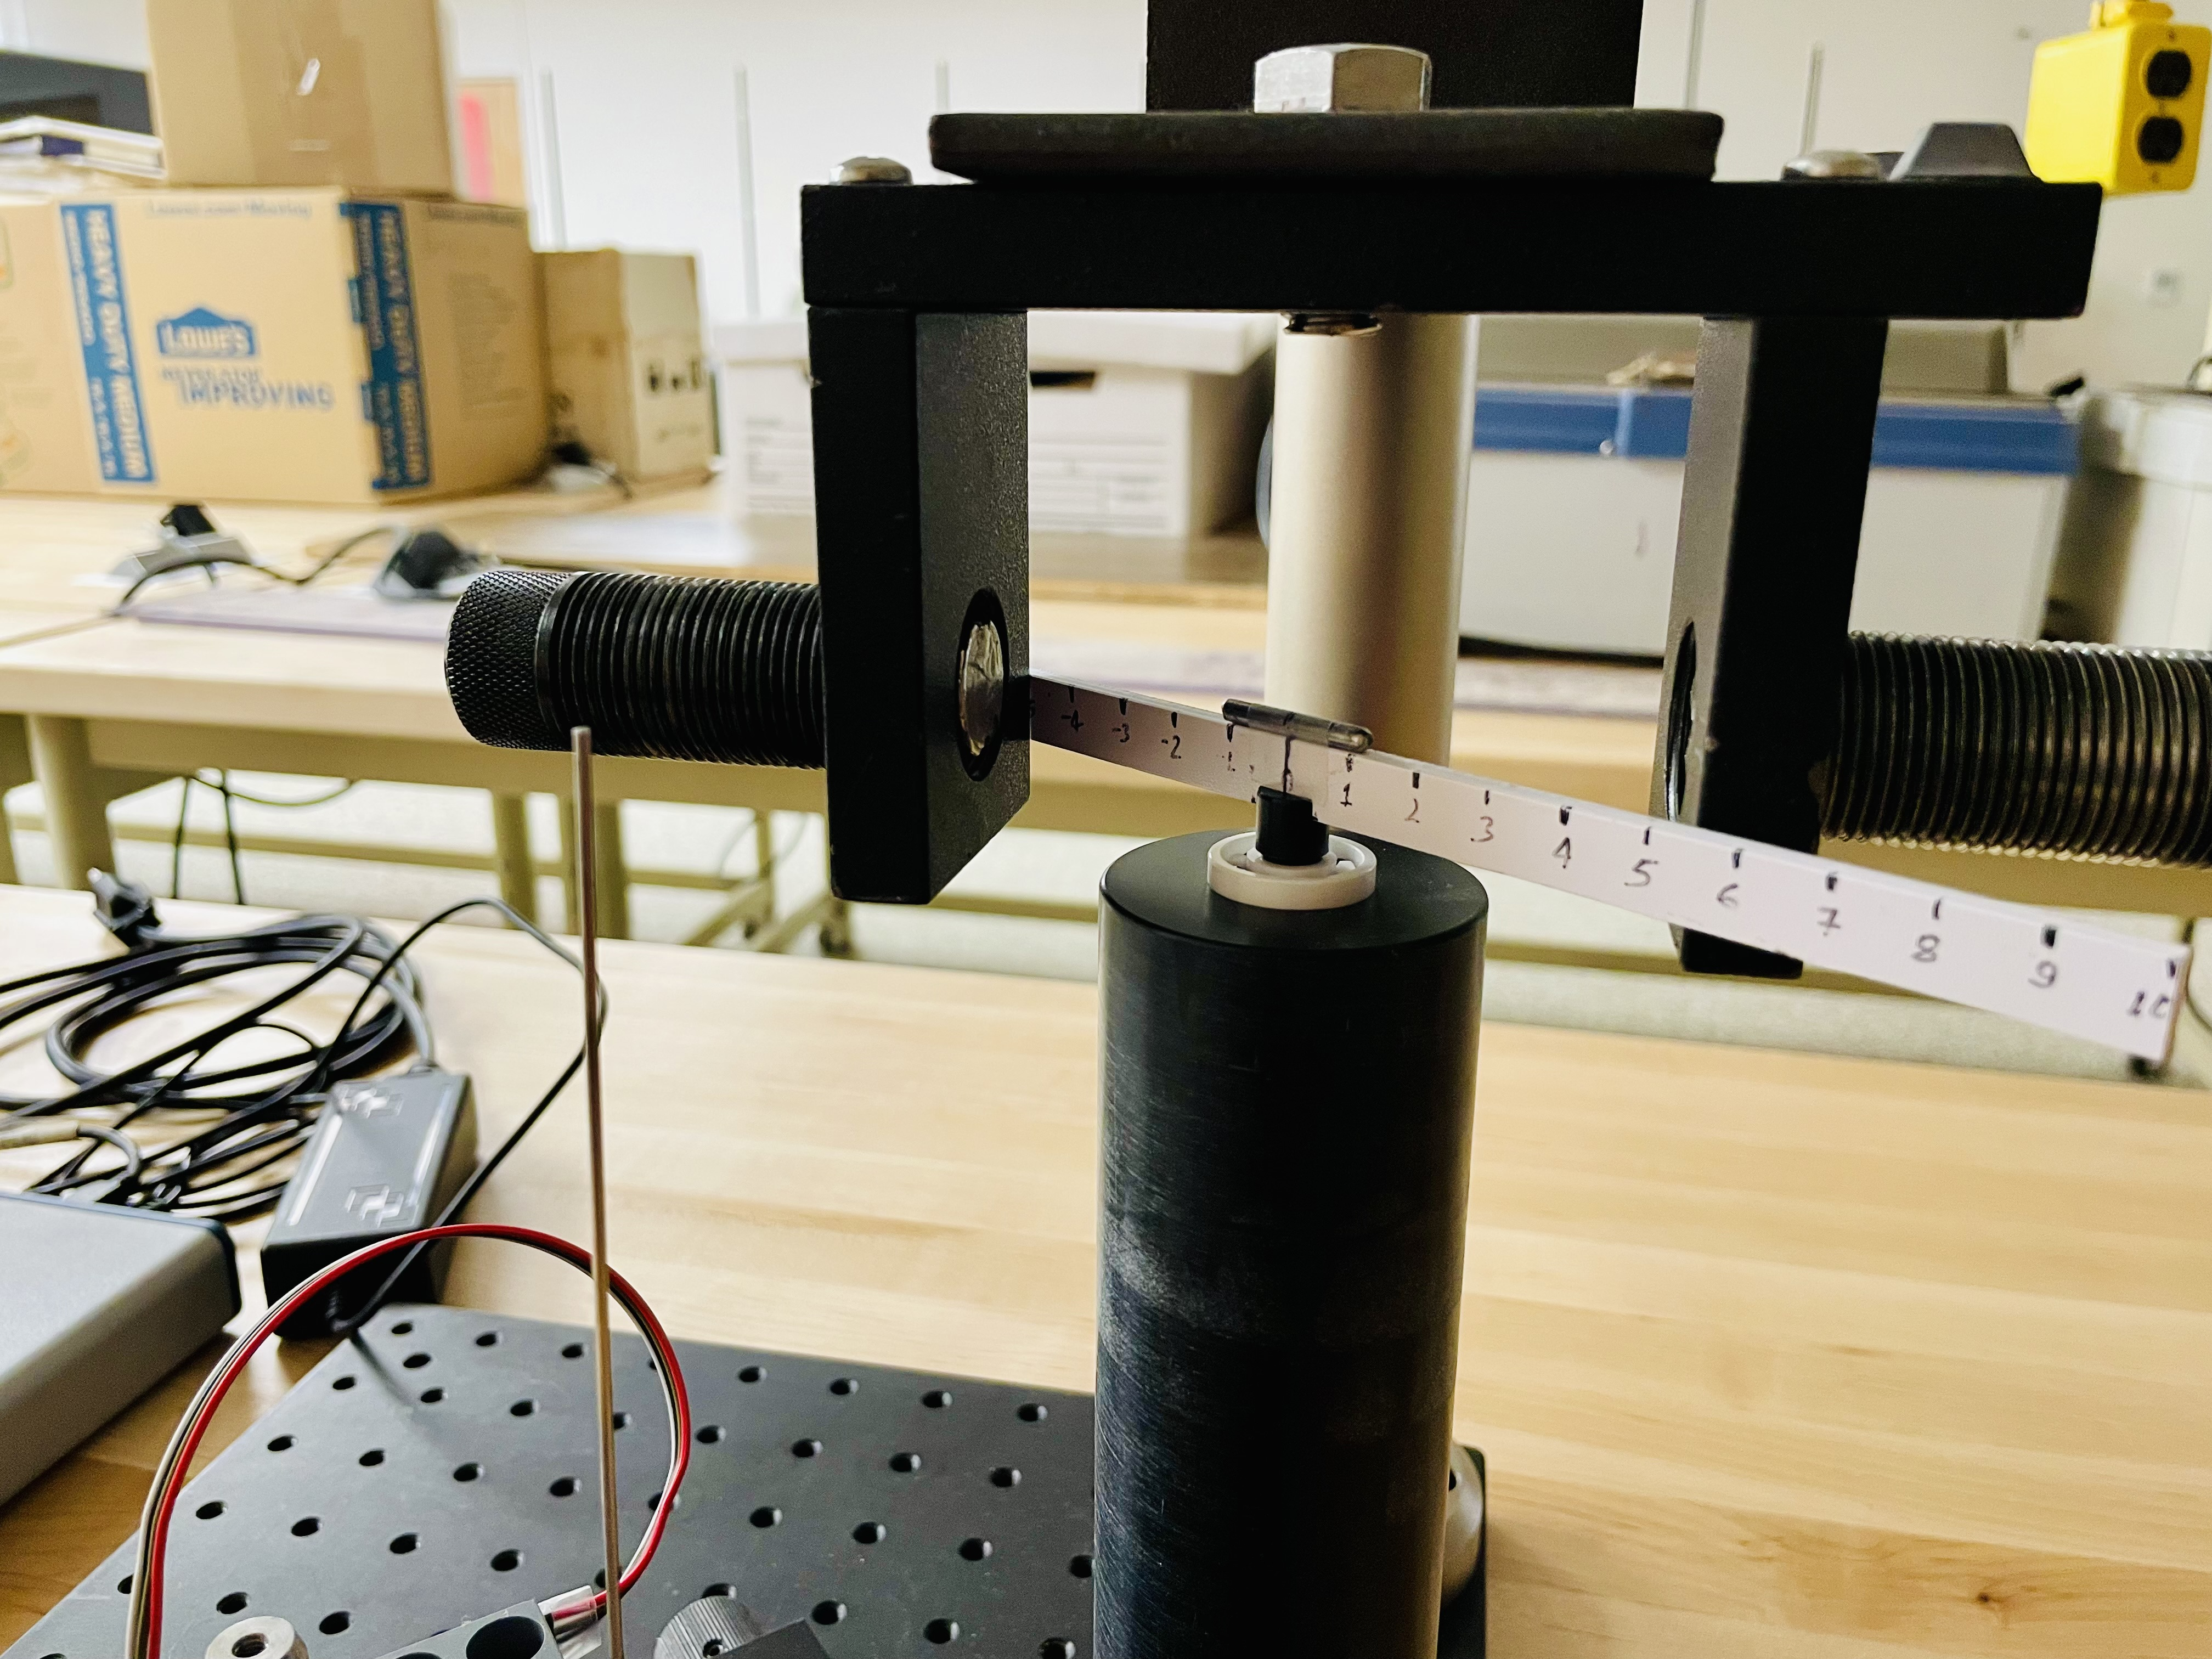
\includegraphics[width=\textwidth]{Assests/torquesCloseup.jpg}
		\subcaption{Close up to the neodymium magnets and test sample (cylindrical metallic piece) were torques are applied.}
	\end{minipage}
	\caption{Implementation of the apparatus in the laboratory setting.}
	\label{fig:torqueDevice}
\end{figure}
